\documentclass[11pt]{article}
\usepackage{acl}

\usepackage{times}
\usepackage{latexsym}
\usepackage[T1]{fontenc}
\usepackage[utf8]{inputenc}
\usepackage{microtype}
\usepackage{inconsolata}
\usepackage{graphicx}
\usepackage{booktabs}
\usepackage{amsmath}
\usepackage{amsfonts}
\usepackage{multirow}
\usepackage{url}
\usepackage{tikz}
\usetikzlibrary{arrows.meta, positioning, fit, calc, backgrounds}

% Okabe-Ito Color Palette (Strict RGB)
\definecolor{oiBlue}{RGB}{0,114,178}
\definecolor{oiOrange}{RGB}{213,94,0}
\definecolor{oiGreen}{RGB}{0,158,115}
\definecolor{oiGray}{RGB}{110,110,110}

\emergencystretch=1.5em

\title{Causal Confidence Halting for Frozen Recursive Sequence Models}

\author{Anonymous Authors}

\begin{document}
\maketitle

\begin{abstract}
We study runtime control of frozen recursive sequence models, where a latent state is refined up to three times before each output token. Most tokens already carry the correct prediction after the base step. Adaptive Computation Time and later halting methods train a gate inside the network, so their savings are predicted exit depths rather than executed calls, and a frozen model admits no gate to train. We present causal confidence halting, a two-stage threshold that stops a token on confidence using only signals available before the refinement it gates. Because high-confidence tokens are stable across depths, stopping there preserves the prediction a deeper step would have produced. On COGS with a frozen GRU encoder--decoder, the threshold retains exact-match accuracy while cutting executed calls to 25.7\% of the deepest baseline on two seeds; on the third seed it improves accuracy by 1.86pp at 52.1\% of the calls. A preregistered confidence-bound criterion confirms non-inferiority on all three seeds, and runtime interception verifies every counted call. At fixed depth, evolutionary step-size policies outperform the original update by up to $+2.1$pp at constant compute. We release the instrumented executor, per-evaluation search logs, and the full confirmation protocol.
\end{abstract}

\section{Introduction}
\label{sec:intro}

Recursive sequence models reapply a refinement operator to a latent state so that later iterations can repair earlier mistakes \citep{graves2016adaptive,dehghani2019universal}. On COGS semantic parsing \citep{kim2020cogs} with a frozen GRU encoder--decoder, the benefit is uneven because 87--91\% of examples keep their prediction across the initial refinement while only 5--9\% are repaired by it. Running the deepest configuration for every token therefore spends most of its compute on tokens that need no further work.

Adaptive Computation Time allocates variable thinking steps through a learned halting unit \citep{graves2016adaptive}, PonderNet learns a probabilistic halting distribution \citep{banino2021ponder}, and depth-adaptive transformers exit per layer or per head \citep{elbayad2020depth,schuster2022calm}. These results assume the network can be retrained, and they express savings as a function of predicted exit depth. A frozen model admits neither assumption. No halting parameters can be fitted, and a predicted depth is not evidence that a call was skipped. The gap between predicted and executed compute is exactly where an adaptive method can report a saving it never delivered.

\begin{figure*}[t]
\centering
\resizebox{\textwidth}{!}{%
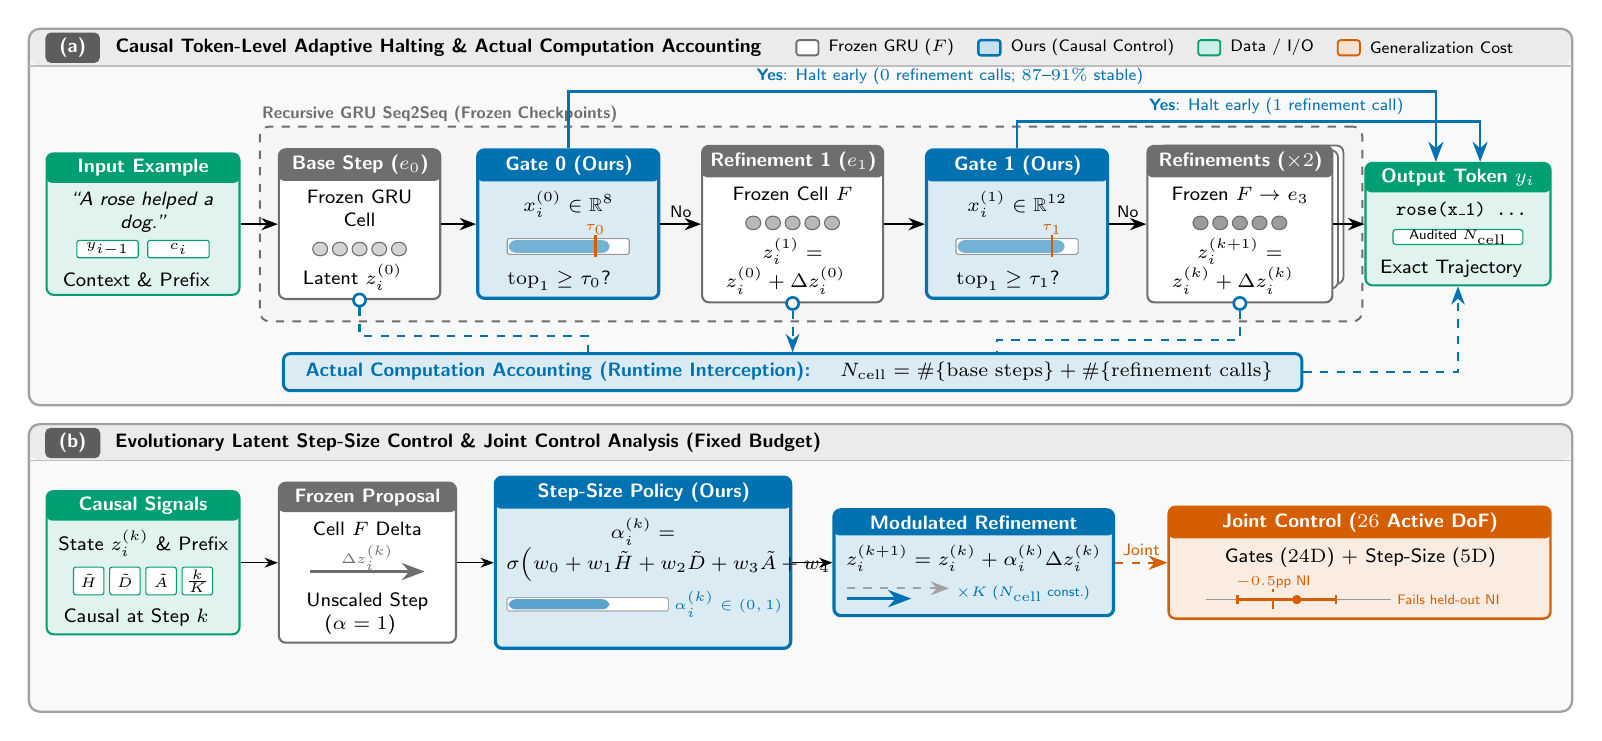
\begin{tikzpicture}[
    font=\sffamily\fontsize{6.8pt}{8.2pt}\selectfont,
    >=Stealth,
    line width=0.65pt,
    % Card Styles
    cardBlue/.style={
        draw=oiBlue, fill=oiBlue!14,
        line width=1.15pt, rounded corners=2.5pt, inner sep=0pt
    },
    cardGray/.style={
        draw=oiGray, fill=white,
        line width=0.75pt, rounded corners=2.5pt, inner sep=0pt
    },
    cardGreen/.style={
        draw=oiGreen, fill=oiGreen!12,
        line width=0.75pt, rounded corners=2.5pt, inner sep=0pt
    },
    cardOrange/.style={
        draw=oiOrange, fill=oiOrange!12,
        line width=0.85pt, rounded corners=2.5pt, inner sep=0pt
    },
    hdr/.style={
        font=\sffamily\fontsize{6.6pt}{7.8pt}\selectfont\bfseries,
        text=white, align=center, inner xsep=2pt, inner ysep=2.2pt,
        rounded corners=1.8pt
    },
    probe/.style={
        circle, draw=oiBlue, fill=white, line width=0.95pt,
        minimum size=4.4pt, inner sep=0pt
    },
    panelBadge/.style={
        font=\sffamily\fontsize{7pt}{8pt}\selectfont\bfseries,
        text=white, fill=oiGray!85!black, rounded corners=2pt, inner xsep=5pt, inner ysep=2pt
    },
    panelTitle/.style={
        font=\sffamily\fontsize{7.5pt}{9pt}\selectfont\bfseries,
        text=black, inner sep=0pt
    },
    tag/.style={font=\sffamily\fontsize{5.8pt}{6.8pt}\selectfont, inner sep=1pt}
]

% Two-tone Header Card Macro
\newcommand{\richcard}[7]{
    \node[#4] (#1) at (#2) {
        \begin{minipage}{#3}
            \centering
            \tikz{\node[hdr, fill=#5, minimum width=#3, text width=\dimexpr#3-4pt\relax] {#6};}\\[-0.5pt]
            \begin{minipage}{\dimexpr#3-8pt\relax}
                \vspace{3pt}\centering #7 \vspace{3pt}
            \end{minipage}
        \end{minipage}
    };
}

\def\xLeft{-0.25}
\def\xRight{19.35}

% ==============================================================================
% PANEL (a) CONTENT
% ==============================================================================
\node[panelBadge, anchor=west] (badgeA) at (-0.05, 5.02) {(a)};
\node[panelTitle, right=5pt of badgeA] (titleA) {Causal Token-Level Adaptive Halting \& Actual Computation Accounting};

% Legend placed directly after titleA with normal spacing
\node[draw=oiGray, fill=white, minimum width=8pt, minimum height=5.5pt, inner sep=0pt, rounded corners=1pt, right=12pt of titleA] (l1) {};
\node[tag, right=2pt of l1] (l1t) {Frozen GRU ($F$)};
\node[draw=oiBlue, fill=oiBlue!22, line width=0.9pt, minimum width=8pt, minimum height=5.5pt, inner sep=0pt, rounded corners=1pt, right=7pt of l1t] (l2) {};
\node[tag, right=2pt of l2] (l2t) {Ours (Causal Control)};
\node[draw=oiGreen, fill=oiGreen!18, minimum width=8pt, minimum height=5.5pt, inner sep=0pt, rounded corners=1pt, right=7pt of l2t] (l3) {};
\node[tag, right=2pt of l3] (l3t) {Data / I/O};
\node[draw=oiOrange, fill=oiOrange!18, minimum width=8pt, minimum height=5.5pt, inner sep=0pt, rounded corners=1pt, right=7pt of l3t] (l4) {};
\node[tag, right=2pt of l4] (l4t) {Generalization Cost};

\def\yA{2.78}

% 1. Input Card (Green)
\richcard{inA}{1.20, \yA}{2.45cm}{cardGreen}{oiGreen}{Input Example}{
    \textit{``A rose helped a dog.''}\\[2.5pt]
    \tikz{
        \foreach \x/\lbl in {0/$y_{i-1}$, 0.90/$c_i$} {
            \draw[draw=oiGreen, fill=white, rounded corners=0.8pt] (\x,0) rectangle ++(0.78, 0.22);
            \node[font=\sffamily\fontsize{5.3pt}{5.3pt}\selectfont] at (\x+0.39, 0.11) {\lbl};
        }
    }\\[2pt]
    Context \& Prefix
}

% 2. Base Step e_0 (Gray)
\richcard{baseA}{3.95, \yA}{2.05cm}{cardGray}{oiGray}{Base Step ($e_0$)}{
    Frozen GRU Cell\\[2.5pt]
    \tikz{
        \foreach \k in {0,1,2,3,4} {
            \draw[draw=oiGray, fill=oiGray!30] (\k*0.25,0) rectangle ++(0.19, 0.17);
        }
    }\\[2pt]
    Latent $z_i^{(0)}$
}

% 3. Gate 0 (Blue - Ours)
\richcard{gate0}{6.60, \yA}{2.30cm}{cardBlue}{oiBlue}{Gate 0 (Ours)}{
    $x_i^{(0)} \in \mathbb{R}^8$\\[1.5pt]
    \tikz{
        \node[font=\sffamily\fontsize{5.2pt}{5.2pt}\selectfont, text=oiOrange, anchor=south] at (1.12, 0.24) {$\tau_0$};
        \draw[draw=oiGray!70, fill=white, rounded corners=0.6pt] (0,0) rectangle (1.55, 0.20);
        \fill[oiBlue!55] (0.02,0.02) rectangle (1.30, 0.18);
        \draw[draw=oiOrange, line width=0.95pt] (1.12, -0.03) -- (1.12, 0.24);
    }\\[1.5pt]
    $\mathrm{top}_1 \ge \tau_0$?
}

% 4. Refinement 1 e_1 (Gray)
\richcard{ref1}{9.45, \yA}{2.30cm}{cardGray}{oiGray}{Refinement 1 ($e_1$)}{
    Frozen Cell $F$\\[2.5pt]
    \tikz{
        \foreach \k in {0,1,2,3,4} {
            \draw[draw=oiGray, fill=oiGray!48] (\k*0.25,0) rectangle ++(0.19, 0.17);
        }
    }\\[2pt]
    $z_i^{(1)} = z_i^{(0)} + \Delta z_i^{(0)}$
}

% 5. Gate 1 (Blue - Ours)
\richcard{gate1}{12.30, \yA}{2.30cm}{cardBlue}{oiBlue}{Gate 1 (Ours)}{
    $x_i^{(1)} \in \mathbb{R}^{12}$\\[1.5pt]
    \tikz{
        \node[font=\sffamily\fontsize{5.2pt}{5.2pt}\selectfont, text=oiOrange, anchor=south] at (1.22, 0.24) {$\tau_1$};
        \draw[draw=oiGray!70, fill=white, rounded corners=0.6pt] (0,0) rectangle (1.55, 0.20);
        \fill[oiBlue!55] (0.02,0.02) rectangle (1.38, 0.18);
        \draw[draw=oiOrange, line width=0.95pt] (1.22, -0.03) -- (1.22, 0.24);
    }\\[1.5pt]
    $\mathrm{top}_1 \ge \tau_1$?
}

% 6. Remaining Refinements x2 -> e_3 (Stacked Gray Cards)
\node[draw=oiGray, fill=white, rounded corners=2.5pt, minimum width=2.35cm, minimum height=50pt] (refK_s2) at (15.27, \yA+0.12) {};
\node[draw=oiGray, fill=white, rounded corners=2.5pt, minimum width=2.35cm, minimum height=50pt] (refK_s1) at (15.20, \yA+0.06) {};
\richcard{refK}{15.13, \yA}{2.35cm}{cardGray}{oiGray}{Refinements ($\times 2$)}{
    Frozen $F \rightarrow e_3$\\[2.5pt]
    \tikz{
        \foreach \k in {0,1,2,3,4} {
            \draw[draw=oiGray, fill=oiGray!68] (\k*0.25,0) rectangle ++(0.19, 0.17);
        }
    }\\[2pt]
    $z_i^{(k+1)} = z_i^{(k)} + \Delta z_i^{(k)}$
}

% 7. Output Card (Green)
\richcard{outA}{17.90, \yA}{2.35cm}{cardGreen}{oiGreen}{Output Token $y_i$}{
    \texttt{rose(x\_1) ...}\\[2.5pt]
    \tikz{
        \draw[draw=oiGreen, fill=white, rounded corners=1pt] (0,0) rectangle (1.65, 0.19);
        \node[font=\sffamily\fontsize{5.3pt}{5.3pt}\selectfont, text=black] at (0.825, 0.095) {Audited $N_{\mathrm{cell}}$};
    }\\[2pt]
    Exact Trajectory
}

% Main Pipeline Arrows
\draw[->] (inA.east) -- (baseA.west);
\draw[->] (baseA.east) -- (gate0.west);
\draw[->] (gate0.east) -- node[tag, above=1pt] {No} (ref1.west);
\draw[->] (ref1.east) -- (gate1.west);
\draw[->] (gate1.east) -- node[tag, above=1pt] {No} (refK.west);
\draw[->] (refK.east) -- (outA.west);

% Top Early-Exit Rails (Blue)
\draw[->, draw=oiBlue, line width=0.95pt]
    (gate0.north) -- ++(0, 0.72) -| node[tag, pos=0.22, above=1pt, text=oiBlue] {\textbf{Yes}: Halt early ($0$ refinement calls; $87\text{--}91\%$ stable)} ([xshift=-8pt]outA.north);

\draw[->, draw=oiBlue, line width=0.95pt]
    (gate1.north) -- ++(0, 0.34) -| node[tag, pos=0.28, above=1pt, text=oiBlue] {\textbf{Yes}: Halt early ($1$ refinement call)} ([xshift=8pt]outA.north);

% Runtime Interception Audit Bus (Bottom)
\node[draw=oiBlue, fill=oiBlue!14, line width=1.05pt, rounded corners=2.5pt, inner xsep=8pt, inner ysep=3.2pt, align=center] (counter) at (9.45, 0.90) {
    \textbf{\textcolor{oiBlue}{Actual Computation Accounting (Runtime Interception):}} \quad
    $N_{\mathrm{cell}} = \#\{\mathrm{base\ steps}\} + \#\{\mathrm{refinement\ calls}\}$
};

% Interception Probes on Frozen Modules
\node[probe] (pr1) at (baseA.south) {};
\node[probe] (pr2) at (ref1.south) {};
\node[probe] (pr3) at (refK.south) {};

\draw[dashed, draw=oiBlue, line width=0.8pt] (pr1) -- ++(0, -0.46) -| ([xshift=-2.6cm]counter.north);
\draw[->, dashed, draw=oiBlue, line width=0.8pt] (pr2) -- (pr2 |- counter.north);
\draw[dashed, draw=oiBlue, line width=0.8pt] (pr3) -- ++(0, -0.46) -| ([xshift=2.6cm]counter.north);
\draw[->, dashed, draw=oiBlue, line width=0.8pt] (counter.east) -| (outA.south);

% Background layers for Panel (a)
\begin{pgfonlayer}{background}
    % Outer Panel (a) Frame
    \draw[draw=oiGray!65, fill=oiGray!4, line width=0.85pt, rounded corners=4pt]
        (\xLeft, 0.48) rectangle (\xRight, 5.26);
    \fill[oiGray!14, rounded corners=3.5pt] (\xLeft+0.02, 4.79) rectangle (\xRight-0.02, 5.24);
    \draw[draw=oiGray!45, line width=0.5pt] (\xLeft, 4.79) -- (\xRight, 4.79);

    % Inner Zone Box for Recursive GRU Seq2Seq
    \node[draw=oiGray, fill=oiGray!7, dashed, line width=0.7pt, rounded corners=3.5pt, inner sep=6.5pt,
          fit=(baseA)(ref1)(refK)(refK_s2),
          label={[tag, text=oiGray, anchor=south west]north west:\textbf{Recursive GRU Seq2Seq (Frozen Checkpoints)}}] {};
\end{pgfonlayer}


% ==============================================================================
% PANEL (b) CONTENT
% ==============================================================================
\node[panelBadge, anchor=west] (badgeB) at (-0.05, 0.00) {(b)};
\node[panelTitle, right=5pt of badgeB] (titleB) {Evolutionary Latent Step-Size Control \& Joint Control Analysis (Fixed Budget)};

\def\yB{-1.52}

% 1. Causal Signals (Green)
\richcard{inB}{1.20, \yB}{2.45cm}{cardGreen}{oiGreen}{Causal Signals}{
    State $z_i^{(k)}$ \& Prefix\\[2.5pt]
    \tikz{
        \foreach \lbl/\x in {$\tilde{H}$/0, $\tilde{D}$/0.46, $\tilde{A}$/0.92, $\frac{k}{K}$/1.38} {
            \node[draw=oiGreen, fill=white, rounded corners=0.8pt, minimum width=11pt, minimum height=10pt, inner sep=0.5pt, font=\sffamily\fontsize{5.4pt}{5.4pt}\selectfont] at (\x+0.2, 0.1) {\lbl};
        }
    }\\[1.5pt]
    Causal at Step $k$
}

% 2. Frozen Cell Update Proposal (Gray)
\richcard{propB}{4.05, \yB}{2.25cm}{cardGray}{oiGray}{Frozen Proposal}{
    Cell $F$ Delta\\[2.5pt]
    \tikz{
        \draw[->, draw=oiGray, line width=1.15pt] (0,0.08) -- (1.45,0.08);
        \node[font=\sffamily\fontsize{5.5pt}{5.5pt}\selectfont, text=oiGray, above] at (0.725, 0.08) {$\Delta z_i^{(k)}$};
    }\\[1.5pt]
    Unscaled Step ($\alpha=1$)
}

% 3. Step-Size Policy (Blue - Ours)
\richcard{stepB}{7.55, \yB}{3.75cm}{cardBlue}{oiBlue}{Step-Size Policy (Ours)}{
    $\alpha_i^{(k)} = \sigma\!\left(w_0 + w_1\tilde{H} + w_2\tilde{D} + w_3\tilde{A} + w_4\frac{k}{K}\right)$\\[2.5pt]
    \tikz{
        \draw[draw=oiGray!60, fill=white, rounded corners=0.6pt] (0,0) rectangle (2.05, 0.17);
        \fill[oiBlue!65] (0.02,0.02) rectangle (1.30, 0.15);
        \node[font=\sffamily\fontsize{5.3pt}{5.3pt}\selectfont, text=oiBlue, anchor=west] at (2.12, 0.085) {$\alpha_i^{(k)} \in (0,1)$};
    }
}

% 4. Modulated Refinement (Blue - Ours)
\richcard{modB}{11.75, \yB}{3.55cm}{cardBlue}{oiBlue}{Modulated Refinement}{
    $z_i^{(k+1)} = z_i^{(k)} + \alpha_i^{(k)}\Delta z_i^{(k)}$\\[2.5pt]
    \tikz{
        \draw[->, draw=oiGray!65, dashed, line width=0.8pt] (0,0.16) -- (1.30,0.16);
        \draw[->, draw=oiBlue, line width=1.2pt] (0,0.03) -- (0.82,0.03);
        \node[font=\sffamily\fontsize{5.3pt}{5.3pt}\selectfont, text=oiBlue, anchor=west] at (1.38, 0.095) {$\times K$ ($N_{\mathrm{cell}}$ const.)};
    }
}

% 5. Joint Control Generalization Failure (Orange - Cost/Failure)
\richcard{jointB}{16.65, \yB}{4.85cm}{cardOrange}{oiOrange}{Joint Control ($26$ Active DoF)}{
    Gates ($24\mathrm{D}$) $+$ Step-Size ($5\mathrm{D}$)\\[2pt]
    \tikz{
        \node[font=\sffamily\fontsize{5.1pt}{5.1pt}\selectfont, text=oiOrange, anchor=south] at (0.85, 0.24) {$-0.5\text{pp}$ NI};
        \draw[draw=oiGray!70] (0,0.10) -- (2.35,0.10);
        \draw[draw=oiOrange, dashed, line width=0.9pt] (0.85, -0.02) -- (0.85, 0.23);
        \draw[draw=oiOrange, line width=1.15pt] (0.40, 0.10) -- (1.65, 0.10);
        \draw[draw=oiOrange, line width=0.9pt] (0.40, 0.04) -- (0.40, 0.16);
        \draw[draw=oiOrange, line width=0.9pt] (1.65, 0.04) -- (1.65, 0.16);
        \fill[oiOrange] (1.15, 0.10) circle (1.7pt);
        \node[font=\sffamily\fontsize{5.3pt}{5.3pt}\selectfont, text=oiOrange, anchor=west] at (2.42, 0.10) {Fails held-out NI};
    }
}

% Panel (b) Flow Arrows
\draw[->] (inB.east) -- (propB.west);
\draw[->] (propB.east) -- (stepB.west);
\draw[->] (stepB.east) -- (modB.west);
\draw[->, dashed, draw=oiOrange, line width=0.85pt] (modB.east) -- node[tag, above=1pt, text=oiOrange] {Joint} (jointB.west);

% Background layers for Panel (b)
\begin{pgfonlayer}{background}
    % Inner Zone Box for Constant-Compute Control
    \node[draw=oiBlue, fill=oiBlue!6, dashed, line width=0.85pt, rounded corners=3.5pt, inner sep=6pt,
          fit=(stepB)(modB)] (zoneB) {};
    \node[tag, text=oiBlue, anchor=north] (zoneBLabel) at ($(zoneB.south)+(0,-1.5pt)$) {\textbf{Fixed-Depth Latent Dynamics Control (Ours)}};

    % Outer Panel (b) Frame (Dynamically encloses zoneBLabel with generous bottom margin)
    \path let \p1 = (zoneBLabel.south) in
        node[draw=oiGray!65, fill=oiGray!4, line width=0.85pt, rounded corners=4pt, inner sep=0pt,
             fit={(\xLeft, \y1-6pt) (\xRight, 0.24)}] (panelBBox) {};
    \fill[oiGray!14, rounded corners=3.5pt] (\xLeft+0.02, -0.22) rectangle (\xRight-0.02, 0.22);
    \draw[draw=oiGray!45, line width=0.5pt] (\xLeft, -0.22) -- (\xRight, -0.22);
\end{pgfonlayer}

\end{tikzpicture}%
}
\caption{\textbf{Causal halting skips redundant refinements while auditing executed calls.} \textbf{(a)} At token $i$, frozen recursive GRU steps ($e_0, e_1, e_3$, gray) are gated by causal confidence thresholds (blue, Ours) using prefix signals ($x_i^{(0)}, x_i^{(1)}$) before unexecuted refinements run, while runtime interception counts true calls ($N_{\mathrm{cell}}$) from input to output (green). \textbf{(b)} At fixed depth, evolutionary step-size policies modulate $\Delta z_i^{(k)}$ via $\alpha_i^{(k)}$, whereas jointly tuned gates and step sizes (orange) do not transfer to held-out data (\S\ref{sec:exp-joint}).}
\label{fig:method_overview}
\end{figure*}

The observation that resolves this gap is local to each token: high-confidence predictions are the ones that stay fixed under refinement, so a confidence score computed before a step tells us whether that step can pay for itself. We present causal confidence halting, a two-stage threshold that reads only signals available before the refinement it gates (Figure~\ref{fig:method_overview}). The earlier gate decides after the base step and the later gate after one refinement; each stops the token when the top prediction clears a preregistered threshold. The executor never computes a step it has decided to skip, so every saved refinement is a call the model truly avoids.

In contrast to learned halting \citep{graves2016adaptive,banino2021ponder} and confidence-based early exit \citep{schuster2022calm}, our procedure changes what is measured as much as what is decided. Prior methods train a gate and infer cost from exit depths; ours freezes the entire model and obtains cost by intercepting the refinement module at runtime. The difference is checkable: forced-depth decoding reproduces frozen trajectories exactly, and a forced stop at the base-step gate executes zero refinement calls. Exact call counting therefore turns a compute ratio into an audited quantity.

On three frozen model seeds of COGS, the two-stage threshold retains the exact-match accuracy of each seed's best fixed depth, using 25.7\% of the deepest baseline's calls on two seeds and 52.1\% of the shallower $e_1$ baseline while gaining 1.86pp EM on the third. A preregistered confidence-bound criterion, applied once to frozen policies on a held-out fold, confirms non-inferiority on all three seeds, and the same frozen policy passes the same criterion unchanged on an untouched development split at compute ratios identical to the third decimal. The same accounting extends to the latent update itself: at fixed depth, evolutionary step-size policies outperform the original update by up to $+2.1$pp. Halting and step-size control are thus measured on a single scale of actually executed calls.

Our stance follows from where the gains come from. On frozen models, the controller-complexity budget is better spent on accounting and confirmation than on richer controllers, because the halting decision is already determined by a signal the base step emits. We therefore study two control dimensions, whether to continue and how to update, and keep them separate so that fixed-depth experiments isolate latent dynamics at constant compute before joint policies are tested on the accuracy--compute frontier of Table~\ref{tab:frontier}. The mechanism, the equal-budget comparisons, and the confirmation protocol follow in the next two sections.

\section{Related Work}
\label{sec:related}

\paragraph{Adaptive computation and early exit.}
Adaptive Computation Time allocates variable thinking steps to recurrent networks with a learned halting unit \citep{graves2016adaptive}; PonderNet learns a probabilistic halting distribution \citep{banino2021ponder}; the Universal Transformer applies depth-adaptive self-attention \citep{dehghani2019universal}, and depth-adaptive transformers exit per layer or per head \citep{elbayad2020depth}. Confidence-based early exit with calibrated scores matches instance complexity to model depth \citep{schwartz2020right}, guarantees consistency between early-exit and full-model predictions \citep{schuster2021cats}, and, closest to our token-level setting, allocates compute per generation timestep in language modeling with sequence-level risk control \citep{schuster2022calm}. Each of these methods fits a gate or a halting distribution, whereas our model is frozen and no halting parameters are trained. All reported compute is the exact count of executed refinement calls, obtained by runtime interception. Anytime and meta-reasoning approaches trade deliberation against cost in a similar spirit \citep{zilberstein1996anytime}.

\paragraph{Recursive and iterative refinement.}
Repeated application of a transformation to a latent state underlies iterative deepening in sequence transduction, from learned halting in recurrent models \citep{graves2016adaptive} to repeated transformer passes \citep{dehghani2019universal}. The empirical structure we exploit is that most examples are stable under additional iterations and a small fraction are repaired. We quantify it as four-way depth transitions (repair, harm, preserve, unresolved) and use the transition counts to design the stopping criterion.

\paragraph{Evolutionary computation for neural control.}
EC has been applied to neural weights (neuroevolution) \citep{stanley2019designing} and to controller optimization \citep{eiben2015introduction}. We restrict EC to a five-dimensional step-size policy on a frozen model, which separates search from representation learning. Our random-search control follows the recommendation that optimizer claims require equal-budget baselines \citep{eiben2015introduction}; our ablations test which feature group actually carries the gain.

\paragraph{Confirmation protocols.}
Cluster-robust bootstrap is standard for grouped data \citep{cameron2015practitioner}. We adopt a preregistered non-inferiority criterion: the lower 95\% confidence bound of the accuracy difference must be $\geq -0.5$pp. We evaluate frozen policies once on a held-out fold, following preregistration practice in empirical sciences. The confidence-bound rule and the confirmation stage matter because point-estimate classifications and inner-subset optima both overstate reliability in our own results.

\section{Method}
\label{sec:method}

Runtime control in this paper has two parts: a halting gate decides which refinements to execute, and a step-size policy decides how strongly each executed refinement moves the latent state. Both read only causally available signals from a frozen GRU encoder--decoder, and both are measured by the same counter of executed cell calls. This section defines the base model, the gate, the counter, and the two policy families (Figure~\ref{fig:method_overview}); \S\ref{sec:experiments} evaluates them against per-seed fixed-depth baselines.

\subsection{Recursive GRU Seq2Seq Model}
\label{sec:model}
To make the control problem explicit, we first fix the model whose refinement steps are gated. The model is a GRU encoder--decoder \citep{cho2014gru,sutskever2014seq2seq} in which, at output position $i$, a base step produces a latent state $z_i^{(0)}$ (depth $e_0$). Up to $K{=}3$ refinement steps may follow, each applying a frozen GRU cell $F$ to the current latent:
\begin{equation}
\begin{aligned}
\Delta z_i^{(k)} &= F\!\left(\big[\,\mathrm{emb}(y_{i-1});\,c_i;\right.\\
 &\qquad\left. e_{\mathrm{soft}}(z_i^{(k)})\,\big],\, z_i^{(k)}\right)-z_i^{(k)},\\
z_i^{(k+1)} &= z_i^{(k)} + \Delta z_i^{(k)},
\end{aligned}
\label{eq:refine}
\end{equation}
where $c_i$ is the encoder context, $e_{\mathrm{soft}}(z)$ the expected embedding under the current output distribution, and $k \in \{0,\dots,K{-}1\}$ indexes refinement steps (depth $e_1$ after one step, $e_3$ after three). Six checkpoints (two model families $\times$ three seeds $s \in \{0,1,2\}$) are frozen; all experiments use family R2.

\paragraph{Empirical depth structure.}
On the gate-training split ($n{=}2{,}419$ per seed), the transition between depths $e_0 \rightarrow e_1$ decomposes into \emph{preserve} (both correct; 87--91\%), \emph{repair} (wrong$\rightarrow$correct; 5--9\%), \emph{unresolved} (both wrong; 3--5\%), and \emph{harm} (correct$\rightarrow$wrong; 0.12--0.25\%). The repair-to-harm ratio of roughly 20--70:1 means recursion is nearly harmless but benefits a minority of examples, which is exactly the structure under which conservative stopping is safe.

\subsection{Causal Token-Level Adaptive Halting}
\label{sec:halting}
Halting needs a decision that is available before the cost it avoids is incurred. At each token, after the base step (and again after the first refinement), a gate decides whether to stop. The decision at each gate may only use signals computed \emph{before} the refinements it gates; the executor never computes a step whose cost is not incurred. Gate~0 (after $e_0$) uses
\begin{equation}
\begin{aligned}
\mathbf{x}^{(0)}_i = \big[ &\mathrm{top}_1,\ \mathrm{margin},\ H,\ \overline{\mathrm{top}}_1,\\
 &p_{75}(H_{\mathrm{hist}}),\ i,\ \mathrm{Var}(\mathrm{top}_1),\\
 &\mathbb{1}[\mathrm{EOS}]\,\big] \in \mathbb{R}^8,
\end{aligned}
\label{eq:gate0}
\end{equation}
where $H$ is the entropy of the current predictive distribution and the remaining entries summarize the decoded prefix; refinement proceeds iff $\sigma(\mathbf{w}_0^\top \mathbf{x}^{(0)}_i + b_0) \geq \tau_0$. Gate~1 (after $e_1$) uses an analogous 12-dimensional vector that also carries the same-state deltas $\Delta\mathrm{top}_1$, $\Delta H$, $\Delta\mathrm{margin}$ and $\lVert z^{(1)}-z^{(0)}\rVert$, and gates the remaining two refinements. The threshold policy in our headline results is the special case ``stop iff $\mathrm{top}_1 \geq \tau$'' with $(\tau_0,\tau_1)=(0.85,0.90)$, preregistered before any evaluation.

\subsection{Actual Computation Accounting}
\label{sec:ncell}
A halting claim is only as strong as the counter behind it, so the compute metric counts calls rather than depths. The metric is
\begin{equation}
N_{\mathrm{cell}} = \#\{\text{base steps}\} + \#\{\text{refinement calls}\},
\label{eq:ncell}
\end{equation}
summed over a corpus and reported relative to the frozen per-seed best fixed depth (\S\ref{sec:setup}). Correctness is enforced by unit tests (forced stop/continue at each gate yields exactly 0/1/3 refinements per token) and by runtime interception that wraps the refinement module and asserts the counter equals the true call count; forced-depth decoding reproduces frozen training-time trajectories exactly (60/60 samples per depth).

\subsection{Evolutionary Latent Step-Size Control}
\label{sec:alpha}
Separately from halting, we ask whether the update magnitude itself should be input-dependent. We replace \eqref{eq:refine} with
\begin{equation}
\begin{aligned}
z_i^{(k+1)} &= z_i^{(k)} + \alpha_i^{(k)}\,\Delta z_i^{(k)},\\
\alpha_i^{(k)} &= \sigma\!\big(w_0 + w_1 \tilde H + w_2 \tilde D\\
 &\qquad + w_3 \tilde A + w_4\, k/K\big),
\end{aligned}
\label{eq:alpha}
\end{equation}
where $\tilde\cdot$ denotes standardization by statistics frozen from $\alpha{\approx}1$ rollouts of the first 64 examples of the inner training subset, $H$ the current predictive entropy, $D = \lVert\Delta z\rVert_2/\sqrt{d}$ the previous displacement, and $A$ the cosine between consecutive updates. Setting $\alpha \equiv 1$ recovers the original trajectories exactly (verified token-by-token, 128/128 per seed); searches are warm-started from $w_0 = 8$, giving $\alpha \approx 0.9997$ rather than exactly 1. All features are causally available at decision time; no gold labels, oracle outcomes, or future-depth signals are used.

\subsection{Joint Control}
Combining both controllers raises a representation question: the two policies must be decoded by one procedure in which gate decisions precede the refinements they gate and step sizes modulate each executed refinement. A joint policy parameterizes both halting gates (24 dimensions, \S\ref{sec:halting}) and the step-size policy (5 dimensions, \eqref{eq:alpha}), yielding a \emph{nominal} 29-dimensional genotype. Two details shrink the effective dimensionality, and we record them rather than overstate the search space. The end-of-sequence indicator features of both gates are always zero at decision time, because decoding terminates as soon as EOS is predicted, so those two weights never act. The joint path also supplies a constant raw value for the direction-consistency feature $A$; after standardization this leaves the corresponding weight confounded with the step-size intercept rather than inactive. The nominal genotype thus has 29 coordinates, of which 27 are non-inactive, but only 26 are functionally independent degrees of freedom.

\subsection{Statistical Criteria}
\label{sec:stats}
Because a point estimate can clear a margin whose confidence bound falls below it, every claim in \S\ref{sec:experiments} is decided by an interval. All intervals are group-cluster paired bootstrap percentiles \citep{cameron2015practitioner} over structural groups of the task (1{,}000 resamples for development comparisons; 20{,}000 for held-out evaluation, fixed seeds). A policy is \emph{non-inferior} to a baseline iff the \textbf{lower 95\% confidence bound} of the exact-match (EM) difference is $\geq -0.5$pp; point estimates alone do not establish non-inferiority. Search budgets are exactly 336 candidate evaluations per optimizer (including the initial population), with warm starts from the preregistered threshold policy and per-evaluation best-so-far logs.

\section{Experiments}
\label{sec:experiments}

Three questions organize the evaluation, one per control surface. Can a causal confidence threshold remove the compute that the depth transitions say is removable, and does the saving survive an untouched split, a full threshold sweep, and beam decoding? Do input-dependent step sizes improve the latent update when the compute is held constant, and what do the searched policies actually change inside the trajectory? And when halting and step-size control are combined and tuned together, does the combination transfer to data it was never tuned on? Every comparison is decided by the same executed-call counter and the same confidence-bound rule, which keeps the three answers comparable on a single scale.

\subsection{Setup}
\label{sec:setup}
We use the COGS semantic parsing benchmark \citep{kim2020cogs} with a frozen gate split of the training distribution (2{,}419 examples per seed): inner folds (4/5 of groups) supply search fitness on group-balanced subsets (192--256 examples); a held-out fold (fold-4, 645 examples per seed, group-disjoint from the search folds) is used only for one-shot evaluation of frozen policies. Group keys, derived from the logical forms of the full training split, are used for fold construction, group-balanced sampling, and bootstrap resampling, but never as per-sample policy inputs. Per-seed frozen best fixed depths are $e_3, e_3, e_1$ for seeds 0--2. Every EM difference and every compute ratio is relative to that seed's own baseline. The sealed COGS test and generalization sets were never read in any experiment reported here. All decoding is greedy argmax at the gated depth, with teacher forcing reserved for training-time trajectory diagnostics. Optimizers (GA, DE, sep-CMA-ES, random search) share the budget of \S\ref{sec:stats}; the optimizer seed is fixed at 0, so optimizer comparisons are exploratory.

\subsection{Causal Execution and Implementation Validation}
A preregistered engineering audit confirmed: (i) forced-depth decoding matches frozen trajectories exactly (60/60 samples per depth, per seed); (ii) the compute counter equals the true base+refinement call count under runtime interception; (iii) a forced stop at gate 0 executes exactly zero refinement calls; (iv) encoder caching used for throughput leaves all decoded tokens, gate actions, and costs bit-identical. Throughput after caching is 24--42 examples/s on CPU.

\subsection{Adaptive Halting Results (RQ1)}
\label{sec:exp-halting}

\begin{table}[t]
\centering
\footnotesize
\setlength{\tabcolsep}{2.5pt}
\begin{tabular}{llcccc}
\toprule
Seed & Policy & $\Delta$EM (pp) & 95\% CI (pp) & $N_{\mathrm{cell}}$ & NI \\
\midrule
\multirow{4}{*}{$s_0$ / $e_3$} & threshold & $+0.00$ & $[0.00, 0.00]$ & 0.2575 & \checkmark \\
 & GA & $-0.31$ & $[-0.99, 0.00]$ & 0.2563 & $\times$ \\
 & DE & $-0.16$ & $[-0.83, 0.47]$ & 0.2563 & $\times$ \\
 & CMA-ES & $-0.31$ & $[-0.99, 0.00]$ & 0.2568 & $\times$ \\
\midrule
\multirow{4}{*}{$s_1$ / $e_3$} & threshold & $+0.00$ & $[0.00, 0.00]$ & 0.2570 & \checkmark \\
 & GA & $-0.47$ & $[-1.36, 0.00]$ & 0.2537 & $\times$ \\
 & DE & $-0.47$ & $[-1.36, 0.00]$ & 0.2530 & $\times$ \\
 & CMA-ES & $-0.93$ & $[-2.33, -0.14]$ & 0.2553 & $\times$ \\
\midrule
\multirow{4}{*}{$s_2$ / $e_1$} & threshold & $+1.86$ & $[-0.48, 6.82]$ & 0.5212 & \checkmark \\
 & GA & $+2.02$ & $[0.00, 6.95]$ & 0.5103 & \checkmark \\
 & DE & $-0.31$ & $[-1.00, 0.00]$ & 0.5047 & $\times$ \\
 & CMA-ES & $+2.02$ & $[0.00, 6.95]$ & 0.5100 & \checkmark \\
\bottomrule
\end{tabular}
\caption{\textbf{Confidence halting retains exact-match accuracy at a fraction of the executed compute.} Held-out fold ($n{=}645$ per seed), relative to each seed's frozen best fixed depth ($e_3$ for seeds 0--1, $e_1$ for seed 2). NI denotes non-inferiority, decided by the preregistered rule LCB$_{95\%}(\Delta\mathrm{EM}) \geq -0.5$pp, \emph{not} by point estimates; CMA-ES denotes sep-CMA-ES. The threshold policy is non-inferior on all three seeds; only 2 of 9 evolutionary policies pass, although 7 of 9 satisfy the point-estimate margin.}
\label{tab:halting}
\end{table}

Causal confidence halting retains exact-match accuracy at a fraction of the executed compute on all three seeds (Table~\ref{tab:halting}, Table~\ref{tab:frontier}). The two-stage threshold is non-inferior on all three seeds while reducing executed recurrent-cell calls (\S\ref{sec:ncell}) by 74--75\% relative to the deepest baseline (seeds 0--1) and by 48\% relative to the already shallow $e_1$ baseline, which it beats by 1.86pp EM (seed 2). The mechanism is consistent with \S\ref{sec:model}: high-confidence tokens are stable across depths, so stopping on confidence is safe. Equal-budget evolutionary optimizers add at most 2.1\% compute, and only two of the nine evolutionary policies satisfy the preregistered confidence-bound non-inferiority criterion, because most optimizer gains come with EM confidence intervals whose lower bounds fall below $-0.5$pp. GA and sep-CMA-ES converge to identical behavior on $s_2$ and are the two passing policies. On this model the halting problem is essentially solved by the threshold.

How much of this hinges on the particular constants $(0.85, 0.90)$? We swept the full grid $\tau_0, \tau_1 \in \{0.50, 0.60, 0.70, 0.80, 0.85, 0.90, 0.95, 0.99\}$ on the held-out fold and found a plateau, not a tuned optimum: every one of the 40 grid points with $\tau_0 \geq 0.8$ is point-estimate non-inferior on every seed, no grid point reaches EM strictly above the preregistered point on seeds 0--1, and on seed 2 all 64 points gain EM with the preregistered point in the maximum band. Across the non-inferior region the compute ratio varies only between 0.253 and 0.292, so the operating point sits within 1.7\% of the cheapest admissible threshold. Under the preregistered pair, 97.4--97.9\% of tokens stop at the base step, which is where the 74--75\% call reduction comes from; the saving is a property of the model's confidence landscape, not of a delicately chosen cutoff.

Is top-1 confidence even the right signal to gate on? A forced-depth probe labels each token by whether stopping at its current depth reproduces the deepest prediction, and measures how well each causally available signal ranks those labels. Top-1 and margin are near-perfect predictors (direction-aware AUC 0.996--1.000), entropy is close behind (0.992--0.998), and the KL divergence between the two depths' predictive distributions follows at 0.979--0.997. The latent-dynamics readouts are weaker and unstable: the cosine between the base-step displacement and the first refinement displacement barely separates the classes, and the displacement norm even reverses its informative direction across seeds. Sweeping two-stage thresholds over each signal family on the held-out fold confirms the probe. Margin is statistically equivalent to top-1 (minimum non-inferior compute within 0.002, identical EM); entropy reaches the same EM at 3--10\% more calls; KL, cosine, and displacement norms are never cheaper at non-inferior EM. Predictive-distribution readouts subsume latent-dynamics readouts on this model, so the simplest member of the best family is also the right one. A width-4 beam study completes the robustness picture: per-beam causal halting reproduces greedy decoding exactly, with identical EM, identical winner-path call counts, and an executed-call ratio of 0.267--0.273 counting every beam expansion. The saving does not depend on the decoding regime.

\begin{table}[t]
\centering
\footnotesize
\setlength{\tabcolsep}{2.5pt}
\resizebox{\linewidth}{!}{%
\begin{tabular}{llcccc}
\toprule
Seed & Policy & $\Delta$EM (pp) & $N_{\mathrm{cell}}$ ratio & extra saving & NI \\
\midrule
$s_0$ & threshold & $+0.00$ & 0.2575 & --- & \checkmark \\
 & GA (tied with DE) & $-0.31$ & 0.2563 & 0.5\% & $\times$ \\
\midrule
$s_1$ & threshold & $+0.00$ & 0.2570 & --- & \checkmark \\
 & DE & $-0.47$ & 0.2530 & 1.6\% & $\times$ \\
\midrule
$s_2$ & threshold & $+1.86$ & 0.5212 & --- & \checkmark \\
 & sep-CMA-ES & $+2.02$ & 0.5100 & 2.1\% & \checkmark \\
\bottomrule
\end{tabular}%
}
\caption{\textbf{The threshold already sits on the accuracy--compute frontier.} For each seed we contrast the preregistered threshold with the cheapest policy the equal-budget optimizers found. The searched policies buy at most 2.1\% more saving than the threshold and, on seeds 0--1, do not pass the non-inferiority bound that the threshold passes. NI denotes the preregistered rule LCB$_{95\%}(\Delta\mathrm{EM}) \geq -0.5$pp; extra saving is the compute the searched policy removes beyond the threshold, relative to the threshold's own saving. Full policy list in Table~\ref{tab:halting}.}
\label{tab:frontier}
\end{table}

\subsection{Fixed-Depth Evolutionary Latent Control (RQ2)}
\label{sec:exp-latent}

\begin{table}[t]
\centering
\footnotesize
\setlength{\tabcolsep}{1.5pt}
\begin{tabular}{lcccc|ccc}
\toprule
& \multicolumn{4}{c|}{Search (inner EM gain, pp)} & \multicolumn{3}{c}{Ablation (GA, $s_0$)} \\
Seed & RS & GA & DE & CMA & A: $k/K$ & B: $H$ & C: $D,A$ \\
\midrule
$s_0$ & $+0.00$ & $+0.52$ & $+0.52$ & $+0.00$ & $+0.52$ & $+0.00$ & $+0.52$ \\
$s_1$ & $+1.04$ & $+1.56$ & $+1.04$ & $+2.08$ & n/a & n/a & n/a \\
$s_2$ & $+0.52$ & $+0.52$ & $+1.04$ & $+0.00$ & n/a & n/a & n/a \\
\bottomrule
\end{tabular}
\caption{\textbf{Step-size policies improve fixed-depth exact match at constant compute.} Fixed-depth (constant $N_{\mathrm{cell}}$) improvements over the original $\alpha{\approx}1$ update on the inner subset ($n{=}192$); all searches use exactly 336 evaluations, and CMA denotes sep-CMA-ES. A hand-designed linearly decaying schedule ($\alpha_k = 1.0-0.5k/K$, i.e., $[1.0, 0.833, 0.667]$ at depth 3) and fixed $\alpha \in \{0.75, 0.5, 0.25\}$ never exceed the $\alpha{\approx}1$ baseline. Ablations on $s_0$ restrict the policy input to a single feature group; the full-feature GA result corresponds to the GA column.}
\label{tab:latent}
\end{table}

At fixed depth the compute is constant, so any EM change is a pure latent-dynamics effect. Evolutionary step-size policies outperform the original update on all seeds, by up to $+2.08$pp (Table~\ref{tab:latent}, Figure~\ref{fig:latent}). On every seed at least one optimizer beats same-budget random search, but no single optimizer does so consistently: on $s_2$, GA merely matches RS and sep-CMA falls below it. A hand-designed linearly decaying schedule over the three steps and all fixed step sizes fail to exceed the baseline. The feature-group ablations on $s_0$ are decisive: a time-index-only policy (A) and a latent-dynamics-only policy (C, using $D$ and $A$) each reproduce the full-feature GA gain exactly ($+0.52$pp), whereas an entropy-only policy (B) does not ($+0.00$pp). The full five-feature state is never necessary, and since dynamics features alone also suffice, the gain cannot be attributed to a pure time schedule either. Figure~\ref{fig:traj} shows the displacement and direction-consistency statistics that motivate these features.

What did the winning policy actually change? Per-token logs answer directly. The learned $\alpha$ is a schedule in disguise: it damps only the first refinement (mean 0.76 at step 0, at least 0.997 thereafter), leaving the deeper steps untouched. Its predictions differ from the original update only at a handful of late, high-entropy positions, six calls across all 645 held-out examples, and on the inner subset the $+0.52$pp gain amounts to exactly one sequence. The searched gains are therefore concentrated where the model is least certain and the trajectory most nearly balanced, an observation that the confirmation analysis of \S\ref{sec:exp-joint} will sharpen into a general conclusion about searched controllers on frozen models.

\begin{figure}[tb]
\centering
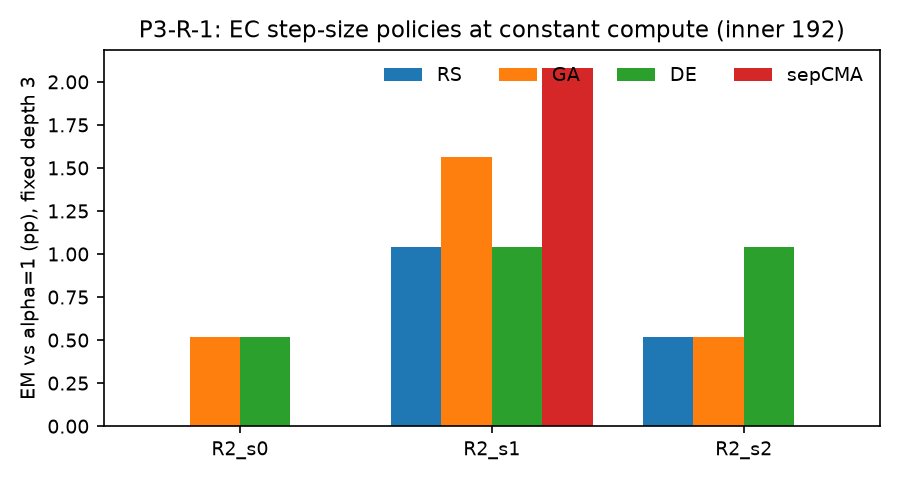
\includegraphics[width=0.8\linewidth]{figures/fig2_p3r1_fixed_depth.png}
\caption{\textbf{Equal-budget evolutionary search improves the latent update at fixed depth.} Inner-subset EM gain (pp) over the original $\alpha{\approx}1$ update for random search and three evolutionary optimizers at equal budgets of 336 evaluations. Feature-group ablations on $s_0$ show that the time index alone and the dynamics pair alone each reproduce the full-feature gain, while entropy alone does not.}
\label{fig:latent}
\end{figure}

\begin{figure}[tb]
\centering
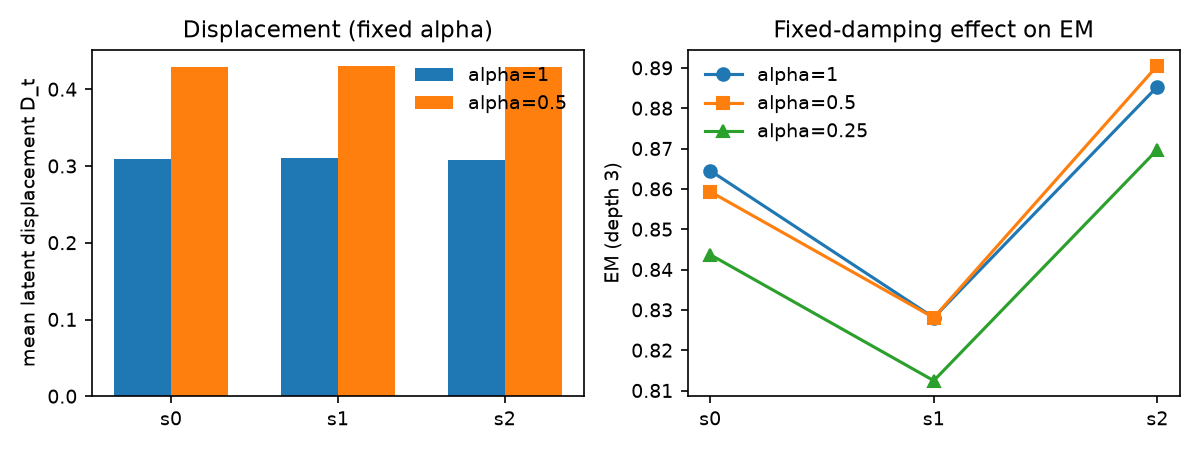
\includegraphics[width=0.9\linewidth]{figures/fig4_p3r0_trajectory.png}
\caption{\textbf{Refinement steps change the latent state less as depth grows.} Per-step displacement and direction consistency of the latent trajectory under fixed damping on the frozen GRU decoder. The concentration of small displacements at later steps motivates a step-size policy that reads entropy, displacement, and direction consistency at decision time.}
\label{fig:traj}
\end{figure}

\subsection{Joint Control and One-Shot Evaluation (RQ3)}
\label{sec:exp-joint}

\begin{table}[t]
\centering
\footnotesize
\setlength{\tabcolsep}{1.5pt}
\begin{tabular}{lcc|ccc}
\toprule
& \multicolumn{2}{c|}{Threshold halting (J1)} & \multicolumn{3}{c}{Joint EC policy (J4)} \\
Seed & $\Delta$EM (pp) & ratio & $\Delta$EM (pp) & 95\% CI (pp) & NI \\
\midrule
$s_0$ & $+0.00$ & 0.2575 & $+0.00$ & $[0.0, 0.0]$ & \checkmark \\
$s_1$ & $+0.00$ & 0.2570 & $-0.31$ & $[-1.0, 0.0]$ & $\times$ \\
$s_2$ & $+1.86$ & 0.5212 & $-0.16$ & $[-0.6, 0.0]$ & $\times$ \\
\bottomrule
\end{tabular}
\caption{\textbf{One-shot confirmation separates retained gains from inner-subset gains.} Held-out fold ($n{=}645$ per seed); NI denotes non-inferiority; CIs are 95\% group-cluster bootstrap intervals of $\Delta$EM (pp) vs.\ the frozen-depth baseline (20{,}000 resamples). J1 passes non-inferiority on all seeds, on $s_2$ only marginally, with 95\% CI $[-0.50, +7.43]$pp, i.e., an LCB of $-0.4975$pp, only 0.0025pp above the bound. The best joint EC policy (selected by inner fitness) fails on $s_1$ and $s_2$, losing on $s_2$ the entire EM gain of the threshold policy (paired $\Delta$EM $-2.02$pp vs.\ J1).}
\label{tab:confirm}
\end{table}

Joint search (27 active dimensions, \S\ref{sec:method}) improves the inner compute ratio over the threshold by only 0.8--5.7\%, so the decisive question is transfer to held-out data (Table~\ref{tab:decomp}). The preregistered one-shot evaluation in Table~\ref{tab:confirm} shows that the threshold policy passes non-inferiority on all three seeds, on $s_2$ only marginally with an LCB of $-0.4975$pp, 0.0025pp above the bound. The jointly optimized policies, despite favorable inner results such as $+0.52$pp at equal cost on $s_1$, do not pass on $s_1$ and $s_2$, and on $s_2$ they give up the entire $+1.86$pp held-out gain of the plain threshold. Inner-subset gains of low-dimensional EC controllers do not transfer to the accuracy--compute frontier.

Why does the combination transfer so poorly when its two components were each tuned under the same budget? Decoding the joint policies with their step-size component pinned to $\alpha{=}1$ isolates the answer (Table~\ref{tab:decomp}). The step-size component contributes nothing: its $\alpha$ never leaves the $\alpha{\approx}1$ warm start, dipping below 0.5 in none of 1{,}429 gated calls, and on the inner folds the searched gates were already no better than the threshold on $s_2$. The held-out loss therefore flows entirely through the searched halting gates, which stop a nearly identical fraction of tokens (gate-0 continue rates 0.01--0.03) but choose slightly different low-confidence tokens to refine. Read together with the per-token analysis of \S\ref{sec:exp-latent}, the pattern is coherent: on a frozen model, a low-dimensional searched controller moves a handful of nearly balanced sequences in whichever direction the inner fold favored, and gains of such controllers do not survive data they were not tuned on. The threshold, in contrast, needed no tuning beyond two preregistered constants.

\begin{table}[t]
\centering
\footnotesize
\setlength{\tabcolsep}{2.5pt}
\resizebox{\linewidth}{!}{%
\begin{tabular}{lccccc}
\toprule
Seed & J1 $\Delta$EM & J4 $\Delta$EM & flips & gates & step size \\
\midrule
$s_0$ & $+0.00$ & $+0.00$ & 0 / 0 & $+0.00$ & $+0.00$ \\
$s_1$ & $+0.00$ & $-0.31$ & 0 / 2 & $-0.31$ & $+0.00$ \\
$s_2$ & $+1.86$ & $-0.16$ & 1 / 14 & $-2.02$ & $+0.00$ \\
\bottomrule
\end{tabular}%
}
\caption{\textbf{Where the joint policy loses.} Held-out fold ($n{=}645$ per seed); J1 is the threshold policy and J4 the jointly tuned policy, with $\Delta$EM in percentage points against each seed's frozen best fixed depth (Table~\ref{tab:confirm}). The last two columns split the J4--J1 gap into the share carried by the searched halting gates and the share carried by the searched step sizes, measured by re-decoding J4 with $\alpha{=}1$; flips count the sequences whose EM changes between J1 and J4, as repair/harm.}
\label{tab:decomp}
\end{table}

\subsection{Fresh-Split Confirmation and Robustness Checks}
\label{sec:exp-fresh}

A confirmation on the held-out fold leaves one residual question: the fold belongs to the training distribution, and its groups were visible to earlier development of the same model line. We therefore evaluated the frozen preregistered policy once more on the official COGS development set ($n{=}3{,}000$), which the frozen checkpoints never trained on and which no experiment reported here had read. The threshold passes the same preregistered non-inferiority criterion on all three seeds, with compute ratios within $0.002$ of the held-out-fold values (Table~\ref{tab:devconfirm}); the measured savings, not merely the operating point, are stable across splits. The official development set is thereafter marked as used.

\begin{table}[t]
\centering
\footnotesize
\setlength{\tabcolsep}{2.5pt}
\resizebox{\linewidth}{!}{%
\begin{tabular}{llccccc}
\toprule
Seed / base & Base EM & Thr.\ EM & $\Delta$EM (pp) & 95\% CI (pp) & ratio & NI \\
\midrule
$s_0$ / $e_3$ & 95.53 & 95.43 & $-0.10$ & $[-0.23, 0.00]$ & 0.2572 & \checkmark \\
$s_1$ / $e_3$ & 97.13 & 97.07 & $-0.07$ & $[-0.17, 0.00]$ & 0.2573 & \checkmark \\
$s_2$ / $e_1$ & 96.77 & 96.97 & $+0.20$ & $[-0.10, +0.51]$ & 0.5182 & \checkmark \\
\bottomrule
\end{tabular}%
}
\caption{\textbf{One-shot confirmation on untouched data.} Official COGS development set ($n{=}3{,}000$; group-cluster paired bootstrap, 20{,}000 resamples), evaluated once with the frozen preregistered threshold and each seed's frozen best fixed depth. The compute ratios match the held-out-fold values (0.2575 / 0.2570 / 0.5212) to the third decimal, so the executed-call savings themselves transfer across splits.}
\label{tab:devconfirm}
\end{table}

\subsection{From Counted Calls to Wall-Clock}
\label{sec:exp-wall}
Executed calls are this paper's currency, but a deployment pays in time, so we measured what the 74\% call reduction buys and what batching takes back. Single-sequence decoding on CPU confirms the accounting end to end: the threshold decodes the held-out fold at roughly a third of the deepest baseline's wall-clock on seeds 0--1 (speedups of $\times$3.2 and $\times$2.8), and at $\times$1.8 on seed 2, whose frozen baseline is the already shallow $e_1$. The gate itself is the residual overhead, since computing the top-1 signal costs roughly half a refinement call (0.46--0.58 equivalents per gated token on our CPU); this is why the realized time ratio sits slightly above the call ratio rather than exactly at it, and why we keep the call counter as the primary metric.

Batching has the larger effect. Serving decodes batches, and within a batch-step every active row pays the maximum depth that any row needs; the gates still act per row, so predictions are unchanged, but part of the saving is spent on rows that did not need the work. Measured with an executor that charges every active row the batch maximum, the executed-call ratio rises from the nominal 0.26 to 0.27 at batch size 4, 0.28--0.29 at 8, and 0.34--0.36 at 32, giving back 4--11\% of the saving at moderate batch sizes and about a third of it at 32, where the wall-clock speedup over the deepest baseline settles at $\times$1.85--1.9 on seeds 0--1. Continuous batching that regroups tokens by needed depth would restore the nominal ratio at the price of scheduling, which is a deployment decision rather than a property of the policy. What the measurement establishes is narrower and more useful: the call counts are honest, the single-sequence speedup is real, and the gap between the two is an accounting choice that a serving stack can make explicit.

\subsection{Does the Mechanism Transfer Beyond the GRU?}
\label{sec:exp-trans}
The halting design leans on two properties of the frozen model: most tokens are already correct after the base step, and confidence identifies them. Neither property is specific to recurrent cells, so we probed transfer with a small recursive Transformer (798{,}633 parameters) trained from scratch under the same protocol. Its decoder applies a causal Transformer base block to produce the per-position latent, then re-applies a separate weight-shared refinement block up to three times with soft feedback in the query; the prediction head is shared across depths, context keys are the emitted tokens alone, and training uses the same multi-depth supervision as the R2 family on the same base split with the same frozen vocabulary.

The pilot reproduces the structure that motivates halting, and then the halting result itself. Forced EM climbs from 68.8\% at $e_0$ to 87.1\% at $e_3$ on the gate-training subset, and the $e_0 \rightarrow e_1$ transition is preserve-dominant (68.0\%) with repair outweighing harm by more than 20:1 (18.4\% vs.\ 0.8\%); on the held-out fold, forced $e_3$ reaches 96.0\%. The preregistered thresholds transfer verbatim at the level of the mechanism: thr(0.85, 0.90) decodes the held-out fold with 0.256 of the deepest baseline's calls at EM within 0.93pp of it (bootstrap CI $[-2.59, +0.27]$pp). What changes is only the operating constant. The Transformer's confidence distribution is shifted, so the last percent needs a higher pair: $(0.99, 0.99)$ recovers the full forced-depth EM of 96.0\% at 0.266 of the calls, and every threshold pair we tried stays inside the 0.25--0.27 compute band. Causal confidence halting with audited executed calls therefore survives a change of refinement operator, with the same counter and the same two-constant policy family; scaling the pilot beyond one seed and one small model remains future work.

\subsection{Release and Verification}
\label{sec:exp-release}
Every experiment above is preregistered before execution, and the released materials make each number checkable. Each search logs all 336 evaluations with best-so-far curves, genotypes, and applied feature masks; per-sample logs (JSONL) and frozen summary files back every table in this paper. A 79-check automated audit validates protocol-level invariants against the raw artifacts, and a separate 170-check manuscript audit cross-verifies, row by row, the numbers printed here (including every confidence-bound classification and the two frontier tables) against the authoritative JSON results. Asset SHA-256 hashes, exact commands, environment versions, and the instrumented executor with its unit tests are included in the release.

\section{Conclusion}
\label{sec:conclusion}
On a frozen recursive GRU model, the reliable way to exploit uneven refinement benefit is a simple, causal, audited confidence threshold. It retains full accuracy at 25.7--25.8\% of the deepest ($e_3$) compute on two seeds and 52.1\% of the shallower $e_1$ baseline compute on the third, and it passes one-shot non-inferiority evaluation on all three seeds, both on the held-out fold and on the untouched development split at compute ratios identical to the third decimal. Because the executor counts every base and refinement call, these ratios are measured savings rather than inferred depths. The same accounting shows where controller complexity pays: equal-budget evolutionary search adds at most 2.1\% compute savings to halting, while fixed-depth step-size policies improve the latent update by up to $+2.1$pp. Our stance is that on frozen models the controller budget is better spent on accounting and confirmation than on richer controllers. Making latent refinement control transferable calls for changing the refinement operator or its training, rather than post-hoc search over a frozen one. We release the causal executor, exact call-count tests, equal-budget controls, mechanism ablations, and the one-shot confirmation protocol as minimum practice for adaptive-computation research.

\section*{Limitations}
Results come from one dataset, one small GRU architecture, and recursion depth $\leq 3$; optimizer seeds are single, so optimizer comparisons are exploratory, and the Transformer pilot of \S\ref{sec:exp-trans} is a single-seed transfer probe rather than a scaled study. Ablations were run on one model seed as preregistered; they show the full input state is unnecessary in that seed, not that individual input features are never useful. Wall-clock latency does not shrink exactly in proportion to call counts because the gate signal costs a fraction of a refinement call itself, and batched execution pays the maximum depth within a batch; both effects are measured in \S\ref{sec:exp-wall}, and call counts remain the primary metric. $N_{\mathrm{cell}}$ counts decoder base and refinement cell invocations only; encoder computation, output projection, softmax, and the gates themselves are not equivalently counted, so it is not a total-FLOPs measure. Group keys used for fold construction, sampling, and bootstrap resampling were derived from the logical forms of the full training split; they never enter any policy as input, but fold structure is not fully independent of the label vocabulary. The sealed COGS test and generalization sets remain unread; the official development set has been used exactly once, as preregistered, for the confirmation of \S\ref{sec:exp-fresh}.

\bibliography{references}

\end{document}
